\documentclass[tikz,border=10pt]{standalone}
% Scale from STYLE METRICS: s = 0.014467 cm per px, origin at circle centre O = I
\usetikzlibrary{calc}
\begin{document}
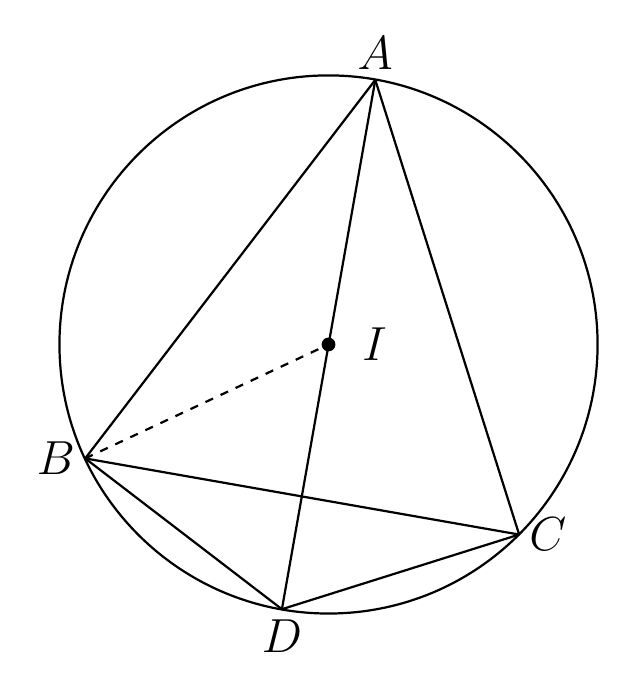
\begin{tikzpicture}[line width=0.8pt, line join=round,
    lbl/.style={font=\fontsize{17}{20.4}\selectfont}]
  % Named coordinates (cm), x=(px-283.7)*s, y=(297.3-py)*s
  \coordinate (O) at (0,0);          % circle centre, also interior point I
  \coordinate (A) at (0.594,3.360);
  \coordinate (B) at (-3.090,-1.447);
  \coordinate (C) at (2.421,-2.414);
  \coordinate (D) at (-0.592,-3.362);
  \coordinate (I) at (0,0);          % I lies on AD (midpoint of diameter)

  % Circle (radius 236.17 px), unchanged
  \draw (O) circle (3.417);

  % Solid chords and diameter AD, unchanged
  \draw (A) -- (B);
  \draw (A) -- (C);
  \draw (B) -- (C);
  \draw (B) -- (D);
  \draw (C) -- (D);
  \draw (A) -- (D);

  % Dashed segment from B to I (ends exactly on AD)
  \draw[dashed] (B) -- (I);

  % Interior point I: filled dot and label to its right
  \fill (I) circle (2.5pt);
  \node[lbl, anchor=west] at ($(I)+(0.3,0)$) {$I$};

  % Point labels outside the circle
  \node[lbl, above] at (A) {$A$};
  \node[lbl, left]  at (B) {$B$};
  \node[lbl, right] at (C) {$C$};
  \node[lbl, below] at (D) {$D$};
\end{tikzpicture}
\end{document}